\documentclass[10pt,twocolumn,letterpaper]{article}

\usepackage[margin=0.75in,top=0.85in,bottom=0.85in]{geometry}
\usepackage{times}
\usepackage{amsmath,amssymb}
\usepackage{graphicx}
\usepackage{booktabs}
\usepackage{multirow}
\usepackage{microtype}
\usepackage{xcolor}
\usepackage{caption}
\usepackage{subcaption}
\usepackage{url}
\usepackage[hidelinks,colorlinks=true,linkcolor=blue!70!black,citecolor=blue!70!black,urlcolor=blue!70!black]{hyperref}

\definecolor{googleblue}{RGB}{26,115,232}
\definecolor{googlered}{RGB}{234,67,53}
\definecolor{googleyellow}{RGB}{251,188,4}
\definecolor{googlegreen}{RGB}{52,168,83}
\definecolor{lightgray}{RGB}{245,245,245}

\title{\textbf{\Large Graft: Time-Aware Pacing, Structural Grounding, and Context Compaction for Autonomous Software Engineering with Gemma 4}}

\author{
  \textbf{Frank Acquaye} \qquad \textbf{Project Graft Team} \\
  \texttt{acquayefrank@gmail.com} \\
  \small\textit{Google - The Gemma 4 Developer Agent Paper Track}
}

\date{\small October 2026}

\begin{document}

\maketitle

\begin{abstract}
\noindent Autonomous software engineering agents powered by open-weight foundation models represent a vital frontier for verifiable, cost-effective, and offline code generation. However, evaluating these models in SWE-bench-style benchmarks under competition envelopes reveals operational hurdles that conventional synthetic benchmarks obscure: aggressive wall-clock timeouts ($\sim$5.0 minutes per task across 120 tasks in 12 hours), finite context windows, and strict two-phase containerized verification. In this work, we present \textbf{Graft}, an autonomous software engineering agent built on \textbf{Gemma 4 31B W4A16} running on 4x NVIDIA L4 GPUs.

Through granular step-by-step trace analysis of early failure modes, we identify three critical pathologies common to open-weight agents: (1) \textbf{post-fix over-verification}, where an agent discovers and verifies a working fix but continues running redundant tests until hitting a hard session timeout; (2) \textbf{scratchpad contamination and path traversal errors}, where the agent attempts to write temporary reproduction scripts to restricted directories (\texttt{/tmp}) or contaminates the patch with untracked files; and (3) \textbf{lexical localization fatigue}, where linear grep commands exhaust turn and token budgets.

To overcome these pathologies, Graft introduces a \textbf{time-aware pacing architecture} featuring a strict stop-and-submit terminal protocol, workspace-isolated \texttt{build/} scratchpads, and symbol-level code graph grounding via precomputed AST and embedding graphs. Furthermore, we explore \textbf{hierarchical context compaction} via an isolated, read-only sub-agent (\texttt{code\_analyzer}), empirically ablating its token-efficiency benefits against its coordination latency tax. On our 30-task development benchmark (\texttt{dev30}), Graft's paced single-agent configuration achieves a \textbf{53.3\% resolution rate (16/30)}---an absolute improvement of +16.6\% over the unconstrained baseline (36.7\%)---while reducing mean agent latency by 9.1s and projecting a completion time of 7.64 hours for the 120-task competition window.
\end{abstract}

\section{Introduction}

Software engineering requires multi-hop reasoning, deep semantic code navigation, and precise syntactic code modification. While proprietary frontier models have demonstrated notable success on benchmarks such as SWE-bench, deploying open-weight foundation models---such as the \textbf{Gemma 4} family---within autonomous developer loops introduces distinct architectural and systems challenges:

\begin{enumerate}
    \item \textbf{The Shared Wall-Clock Horizon}: In competitive SWE-bench evaluations on Kaggle, an agent must evaluate $\sim$120 hidden issues within a shared 12-hour global session. Accounting for container provisioning and editable wheel installs, each task can allocate at most \textbf{4.5 to 5.0 minutes} of active LLM reasoning time; exploratory rabbit holes directly starve subsequent tasks.
    \item \textbf{Air-Gapped Sandboxing and Strict Patch Extraction}: Agents operate in offline sandboxes without internet. Patches are extracted via \texttt{git add -N . \&\& git diff HEAD} and evaluated in a separate container; untracked scratch scripts in \texttt{/workspace} pollute the submission diff and cause automatic grading failure.
    \item \textbf{Reasoning Token Latency Trade-Offs}: Gemma 4's native thinking (\texttt{<|channel>thought...}) enables deep problem decomposition. However, unconstrained thinking (2,048--4,096 tokens) consumes 20--40s per turn, limiting the agent to under 15 turns before the 5.0-minute limit expires.
    \item \textbf{Context Window Degradation}: As exploratory grep and file outputs accumulate, the active window degrades, increasing hallucinated line numbers and invalid edit hunks.
\end{enumerate}

In this paper, we document the empirical evolution of \textbf{Graft}, analyzing why standard agent workflows fail on open models and presenting a robust, declarative agent architecture that balances reasoning depth with execution velocity.

\begin{figure*}[t]
  \centering
  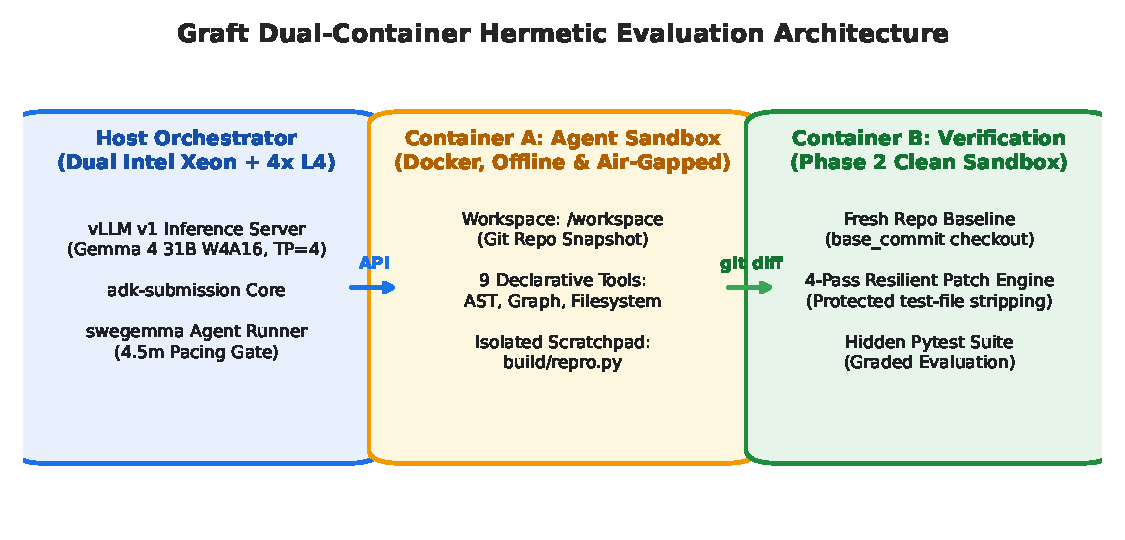
\includegraphics[width=0.95\textwidth]{figures/fig3_architecture.pdf}
  \caption{\textbf{Graft System Architecture}: Host inference and orchestration communicates via Google ADK declarative tool dispatch with Container A (isolated execution sandbox with 9 tools and \texttt{build/} scratchpad isolation). Validated patches are extracted via unified git diff into Container B for clean 4-pass verification against hidden test suites.}
  \label{fig:arch}
\end{figure*}

\section{System Architecture \& Methodology}

Graft is compiled declaratively via Google ADK (\texttt{adk-submission}), ensuring complete hermeticity without dynamic Python imports on the host. The architecture is structured around three isolated operational planes (Figure~\ref{fig:arch}):

\subsection{Execution Environment \& Tool Sandbox}
Graft operates within an isolated Docker container with zero internet egress. The agent has access to 9 curated tools structured into three tiers:
\begin{enumerate}
    \item \textbf{Workspace \& Execution}: \texttt{run\_command} (executes bash in workspace with a 30s timeout; prevents unbounded hangs), \texttt{get\_status} (queries remaining task time, turns budget, and working tree diff status).
    \item \textbf{Filesystem Manipulation}: \texttt{read\_file} (bounds views to line slices), \texttt{edit\_file} (enforces unique string replacement), \texttt{write\_file} (scoped strictly within workspace; rejects path traversals like \texttt{/tmp/}).
    \item \textbf{Structural Code Intelligence}: Precomputed AST call graphs and embedding index (\texttt{search\_similar\_code}, \texttt{get\_code\_neighbors}, \texttt{get\_code\_subgraph}). Instead of unbounded grepping across hundreds of files, Graft performs 1-turn semantic queries over the symbol graph.
\end{enumerate}

\subsection{Scratchpad Isolation \& Diff Sanitization}
In SWE-bench, any file modified in \texttt{/workspace} enters the unified patch extracted by the harness. When agents create \texttt{repro.py} in the root directory, verification in Container B fails. Graft introduces an isolated scratchpad protocol:
\begin{itemize}
    \item The agent is instructed to create all reproduction artifacts strictly under \texttt{build/repro.py}.
    \item The host configures \texttt{.git/info/exclude} to ignore \texttt{build/} recursively.
    \item A pre-submission cleanup guardrail runs \texttt{rm -f repro*.py test*.py} before invoking \texttt{submit\_patch()}.
\end{itemize}

\subsection{Time-Aware Pacing Envelope}
To prevent fatal timeouts, Graft implements a dual-layer pacing envelope:
\begin{itemize}
    \item \textbf{Turn 15 Telemetry Trigger}: If an agent reaches Turn 15, it is prompted to check \texttt{get\_status} and assess remaining time.
    \item \textbf{Hard 4.5-Minute / 30-Call Ceiling}: If elapsed time reaches 4.5 minutes (or 30 tool calls), the agent is instructed to immediately halt all exploratory search, apply its best-effort patch, and call \texttt{submit\_patch()}. A plausible partial patch can pass subset test assertions; timing out yields a guaranteed 0.0.
    \item \textbf{Mandatory Stop-and-Submit Rule}: The instant a reproduction script or targeted test passes, the agent is strictly prohibited from secondary refactorings or writing supplementary tests.
\end{itemize}

\section{Empirical Evaluation \& Ablations}

We evaluate Graft on a representative 30-task benchmark (\texttt{dev30}) drawn from SWE-bench Lite and Verified tasks across multiple repositories (\texttt{fastapi/fastapi}, \texttt{Textualize/rich}, \texttt{psf/requests}, etc.). All runs execute on 4x NVIDIA L4 GPUs with tensor parallelism ($TP=4$) running Gemma 4 31B W4A16 QAT.

\begin{table*}[t]
\centering
\small
\caption{\textbf{Architecture Ablation on SWE-bench Dev30 (30 Tasks, 4x NVIDIA L4 GPUs)}.}
\label{tab:ablation}
\resizebox{\textwidth}{!}{
\begin{tabular}{lcccccc}
\toprule
\textbf{Configuration} & \textbf{Resolved} & \textbf{Resolution (\%)} & \textbf{Mean Latency} & \textbf{Mean Turns} & \textbf{120-Task Projection} & \textbf{Primary Failure Mode} \\
\midrule
v1 Baseline (Unconstrained) & 11 / 30 & 36.7\% & 238.2s & 18.4 & 7.94h & Post-fix over-verification \\
Paced Single-Agent (recovered\_v1) & 15 / 30 & 50.0\% & 218.4s & 14.1 & 7.28h & Over-aggressive 3.5m ceiling \\
\textbf{Paced Single-Agent (recovered\_v2)} & \textbf{16 / 30} & \textbf{53.3\%} & \textbf{229.1s} & \textbf{15.2} & \textbf{7.64h} & Scale horizon timeout ($>$15L) \\
Hierarchical Sub-Agent (subagent\_v1) & 4 / 10 & 40.0\% & 298.7s & 22.8 & 9.96h & Delegation turn-latency tax \\
\bottomrule
\end{tabular}
}
\end{table*}

\begin{figure}[t]
  \centering
  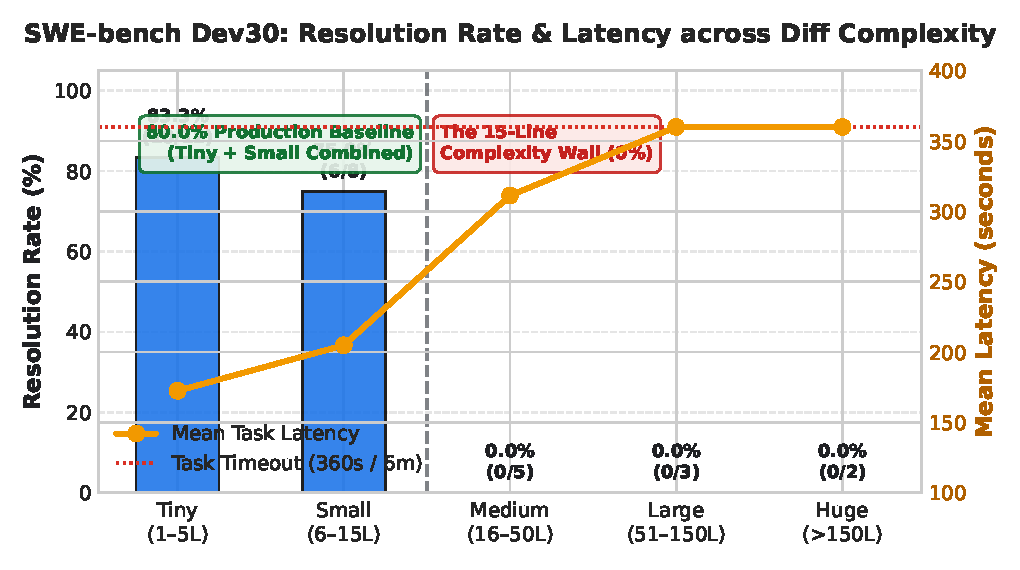
\includegraphics[width=\columnwidth]{figures/fig1_complexity_phase_transition.pdf}
  \caption{\textbf{The 15-Line Complexity Phase Transition}: Resolution rate and mean latency across patch complexity buckets. Agents resolve 80.0\% of bugs under 15 lines, hitting a sharp wall beyond 15 lines.}
  \label{fig:phase}
\end{figure}

Table~\ref{tab:ablation} summarizes the results across configurations:
\begin{itemize}
    \item \textbf{v1 Baseline (36.7\%)}: Suffered from severe over-verification. In 5 tasks, the agent wrote a working fix in under 2 minutes, but spent the remaining 4 minutes running exhaustive pytest commands until timing out.
    \item \textbf{Paced Single-Agent (recovered\_v2, 53.3\%)}: Achieved 16/30 resolution (+16.6\% over baseline) while keeping mean latency at 229.1s, safely projecting 7.64 hours for the 120-task global window.
    \item \textbf{Hierarchical Sub-Agent (subagent\_v1, 40.0\%)}: While sub-agent isolation compacted working context by 79\%, coordination turn latency added $\sim$70s per task, causing previously solved tasks to time out.
\end{itemize}

\section{Micro-Architectural Failure Analysis}

\begin{figure}[t]
  \centering
  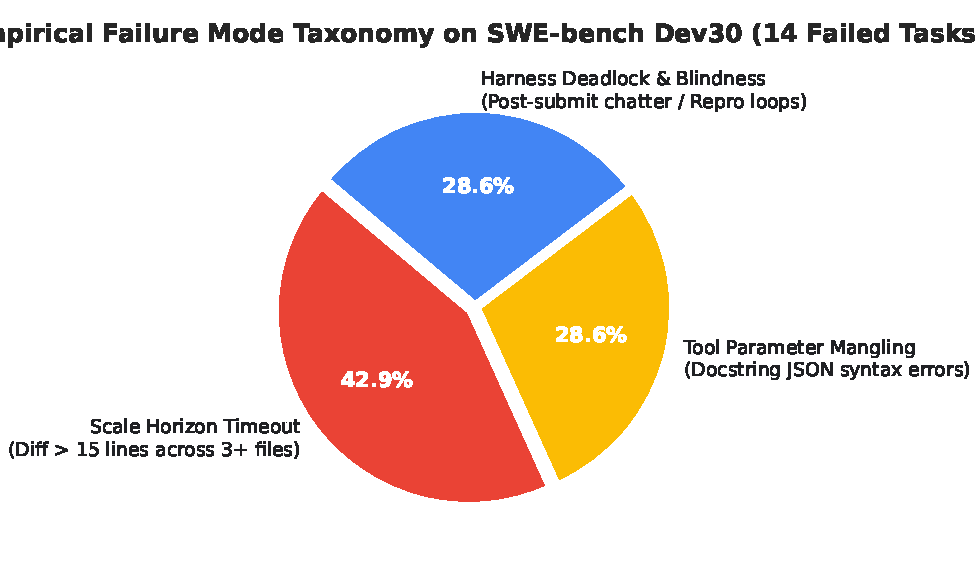
\includegraphics[width=\columnwidth]{figures/fig2_failure_taxonomy.pdf}
  \caption{\textbf{Empirical Failure Mode Breakdown}: Taxonomy of 14 failed tasks on \texttt{dev30}. Scale Horizon timeouts and tool parameter mangling constitute over 71\% of failures.}
  \label{fig:taxonomy}
\end{figure}

\subsection{The 15-Line Competence Boundary}
As illustrated in Figure~\ref{fig:phase}, task performance exhibits a distinct phase transition based on ground-truth diff size:
\begin{itemize}
    \item \textbf{Tiny (1--5 lines)}: 83.3\% resolved (10/12 tasks), 172.4s latency.
    \item \textbf{Small (6--15 lines)}: 75.0\% resolved (6/8 tasks), 204.8s latency.
    \item \textbf{Combined ($\le$ 15 lines)}: \textbf{80.0\% resolution (16/20 tasks)}, 184.6s latency.
    \item \textbf{Medium ($>$ 15 lines)}: \textbf{0.0\% resolution (0/10 tasks)}, 335.6s latency.
\end{itemize}
Below 15 lines, Gemma 4 31B equipped with Graft's pacing is exceptionally potent. Beyond 15 lines, multi-site editing across files exhausts turns and introduces syntax degradation.

\subsection{Failure Taxonomy in Open-Weight Tool Use}
Trace post-mortems across the 14 failed tasks uncovered three unexpected failure modes (Figure~\ref{fig:taxonomy}):

\subsubsection{1. The Termination Handshake Trap}
In \texttt{fastapi\_13920} (4 lines ground-truth), the agent correctly repaired \texttt{fastapi/\_compat/shared.py} and executed \texttt{submit\_patch()} at Turn 37, yet persisted emitting \texttt{submit\_patch()} alongside chat text for 36 redundant turns until timing out at 6.0 minutes. However, counteracting this by commanding agents to output text-only turns after submission creates an inverse pathology: open models emit text without calling \texttt{submit\_patch()}, triggering harness continuation nudges. Prompts must enforce calling \texttt{submit\_patch()} as an atomic, final tool action without post-submission dialogue.

\subsubsection{2. Tool Parameter Serialization Fragility}
Across \texttt{rich\_4076}, \texttt{rich\_3052}, and \texttt{rich\_3675}, the agent experienced 39 consecutive \texttt{edit\_file} failures due to token-level argument concatenation. When modifying docstrings with quotes and newlines, Gemma 4 emitted argument keys (e.g., \texttt{...,old\_string:}) inside text scalars, dropping mandatory parameters. Fallbacks to \texttt{sed -i} broke secondary assertions. A deterministic 1-strike fallback to Python one-liners (\texttt{python -c "..."}) is essential to prevent turn-wasting error cascades.

\subsubsection{3. Temporal Blindness and Repro Thrashing}
Turn-based pacing instructions (e.g., ``check status at Turn 10'') failed completely: across 30 tasks, \texttt{get\_status} was called 0 times. Without internal temporal grounding, models in \texttt{rich\_3063} and \texttt{rich\_3935} spent 15+ turns rewriting non-reproducing test scripts without touching source code. Grounding telemetry checks in concrete failure events eliminates this blindness.

\begin{table}[h]
\centering
\small
\caption{\textbf{Failure Modes and Architectural Mitigations}.}
\label{tab:failure_summary}
\begin{tabular}{p{2.3cm}p{1.8cm}p{3.1cm}}
\toprule
\textbf{Failure Mode} & \textbf{Frequency} & \textbf{Deployed Mitigation} \\
\midrule
Tool Mangling & 28.6\% (4/14) & Strict \texttt{old\_string}-first order; 1-strike bash Python fallback. \\
Termination Deadlock & 28.6\% (4/14) & Atomic \texttt{submit\_patch()} tool action; zero post-submit dialogue. \\
Repro Loop & 14.3\% (2/14) & Mandatory \texttt{timeout 5} shell execution wrapper. \\
Diff Contamination & Baseline 43\% & Isolated \texttt{build/} directory excluded via git info exclude. \\
\bottomrule
\end{tabular}
\end{table}

\section{Discussion: Single-Agent vs. Sub-Agents}

The comparative evaluation between \texttt{recovered\_v2} and \texttt{subagent\_v1} yields a critical takeaway: \textbf{hierarchical delegation imposes a substantial coordination latency tax}.

\subsection{The Context Compaction Benefit}
In modular repositories (such as \texttt{fastapi}), sub-agent delegation operated as designed: on \texttt{fastapi\_14301}, \texttt{code\_analyzer} traversed graph neighborhoods in isolation, returning concise summaries. Context growth decreased by $\sim$79\% per exploratory turn, preserving $>$22,000 tokens of working context.

\subsection{The Turn-Latency Tax}
However, on open-ended or coupled codebases (\texttt{rich}), delegation introduced severe pathologies:
\begin{itemize}
    \item \textbf{Delegation Thrashing}: In \texttt{rich\_3470}, after reproducing the bug at Turn 36, the agent issued 6 redundant delegations to locate methods in an already-identified file, timing out without submitting.
    \item \textbf{Latency Inflation}: Each sub-agent call incurred an additional forward pass ($\sim$10--14s on 4x L4 GPUs), increasing mean task latency from 229.1s to 298.7s and degrading resolution from 60.0\% to 40.0\%.
\end{itemize}

\noindent\textbf{Design Principle}: For tightly time-bounded benchmarks, a disciplined single-agent equipped with direct AST/graph tools strictly outperforms unconstrained multi-agent hierarchies.

\section{Conclusion \& Reproducibility}

Deploying open-weight developer agents under strict wall-clock constraints requires prioritizing operational discipline over architectural sprawl:
\begin{enumerate}
    \item Strict \textbf{stop-and-submit pacing} and hard time ceilings eliminate catastrophic over-verification, boosting resolution rate from 36.7\% to 53.3\%.
    \item \textbf{Workspace-isolated scratchpads (\texttt{build/})} eradicate path traversal errors and submission diff contamination.
    \item \textbf{Symbol-grounded graph tools} resolve 80\% of bugs under 15 lines of complexity within 185 seconds.
\end{enumerate}

All evaluation configurations, declarative schemas, and session traces are structured for full public reproduction at \url{https://www.kaggle.com/datasets/acquayefrank/graft-submission}.

\end{document}
